\documentclass[a4paper,12pt]{article}
\usepackage{amsmath}
\usepackage{graphicx}
\usepackage{enumitem}
\usepackage{booktabs}
\usepackage{listings}
\usepackage{hyperref}

\title{Trade-offs in FRF Measurements}
\author{}
\date{}
\begin{document}

% Cover page information
\begin{center}
    \Large \textbf{Measurement and Data Driven Modeling}\\
    \vspace{0.3cm}
    \LARGE \textbf{Assignment Report}\\
    \vspace{0.5cm}
    \Large \textbf{Trade-offs in FRF Measurements}\\
    \vspace{1cm}
\end{center}

\section*{Objective}
This assignment aims to explore and demonstrate the practical trade-offs between:
\begin{enumerate}
    \item Frequency resolution
    \item Measurement time
    \item Signal-to-Noise Ratio (SNR)
\end{enumerate}
in the context of measuring Frequency Response Functions (FRFs). This understanding is crucial when designing excitation signals for system identification.

\section*{Background}
Measuring accurate FRFs requires balancing three competing factors:
\begin{enumerate}
    \item \textbf{Frequency Resolution}: Higher resolution allows more frequency lines to be distinguished within a given bandwidth.
    \item \textbf{Measurement Time}: Longer signals allow more averaging, reducing random noise.
    \item \textbf{SNR}: The clarity with which excited frequency components emerge from the noise floor.
\end{enumerate}
This trade-off is fundamental and unavoidable in any practical measurement setup. The trade-offs explored in this assignment assume:
\begin{itemize}
    \item The RMS amplitude of the excitation signal is fixed to \(1 \,V\).
    \item The frequency band of interest lies between 5 Hz and 10 Hz.
\end{itemize}

\section*{Multisine Design Summary}
The table below summarizes six example multisines designed to illustrate the trade-offs under different constraints:

\begin{table}[h!]
\centering
\caption{Example Multisine Designs for Each Trade-off Case}
\begin{tabular}{@{}lccc@{}}
\toprule
\textbf{Trade-off Case} & \textbf{Excited Frequencies (Hz)} & \textbf{Period (s)} & \textbf{Notes} \\ \midrule
Fixed Resolution 1 & 5 to 10 Hz (30 lines) & 6 s & Balanced power \\
Fixed Resolution 2 & 5 to 10 Hz (30 lines) & 12 s & Higher SNR \\
Fixed Time 1 & 5 to 10 Hz (30 lines) & 6 s & Baseline \\
Fixed Time 2 & 5 to 10 Hz (60 lines) & 6 s & Finer resolution \\
Fixed SNR 1 & 5 to 10 Hz (30 lines) & 6 s & Target SNR 40 dB \\
Fixed SNR 2 & 5 to 10 Hz (60 lines) & 12 s & Same SNR, more lines \\
\bottomrule
\end{tabular}
\end{table}

\section*{Results and Explanation}

\begin{figure}[h!]
    \centering
    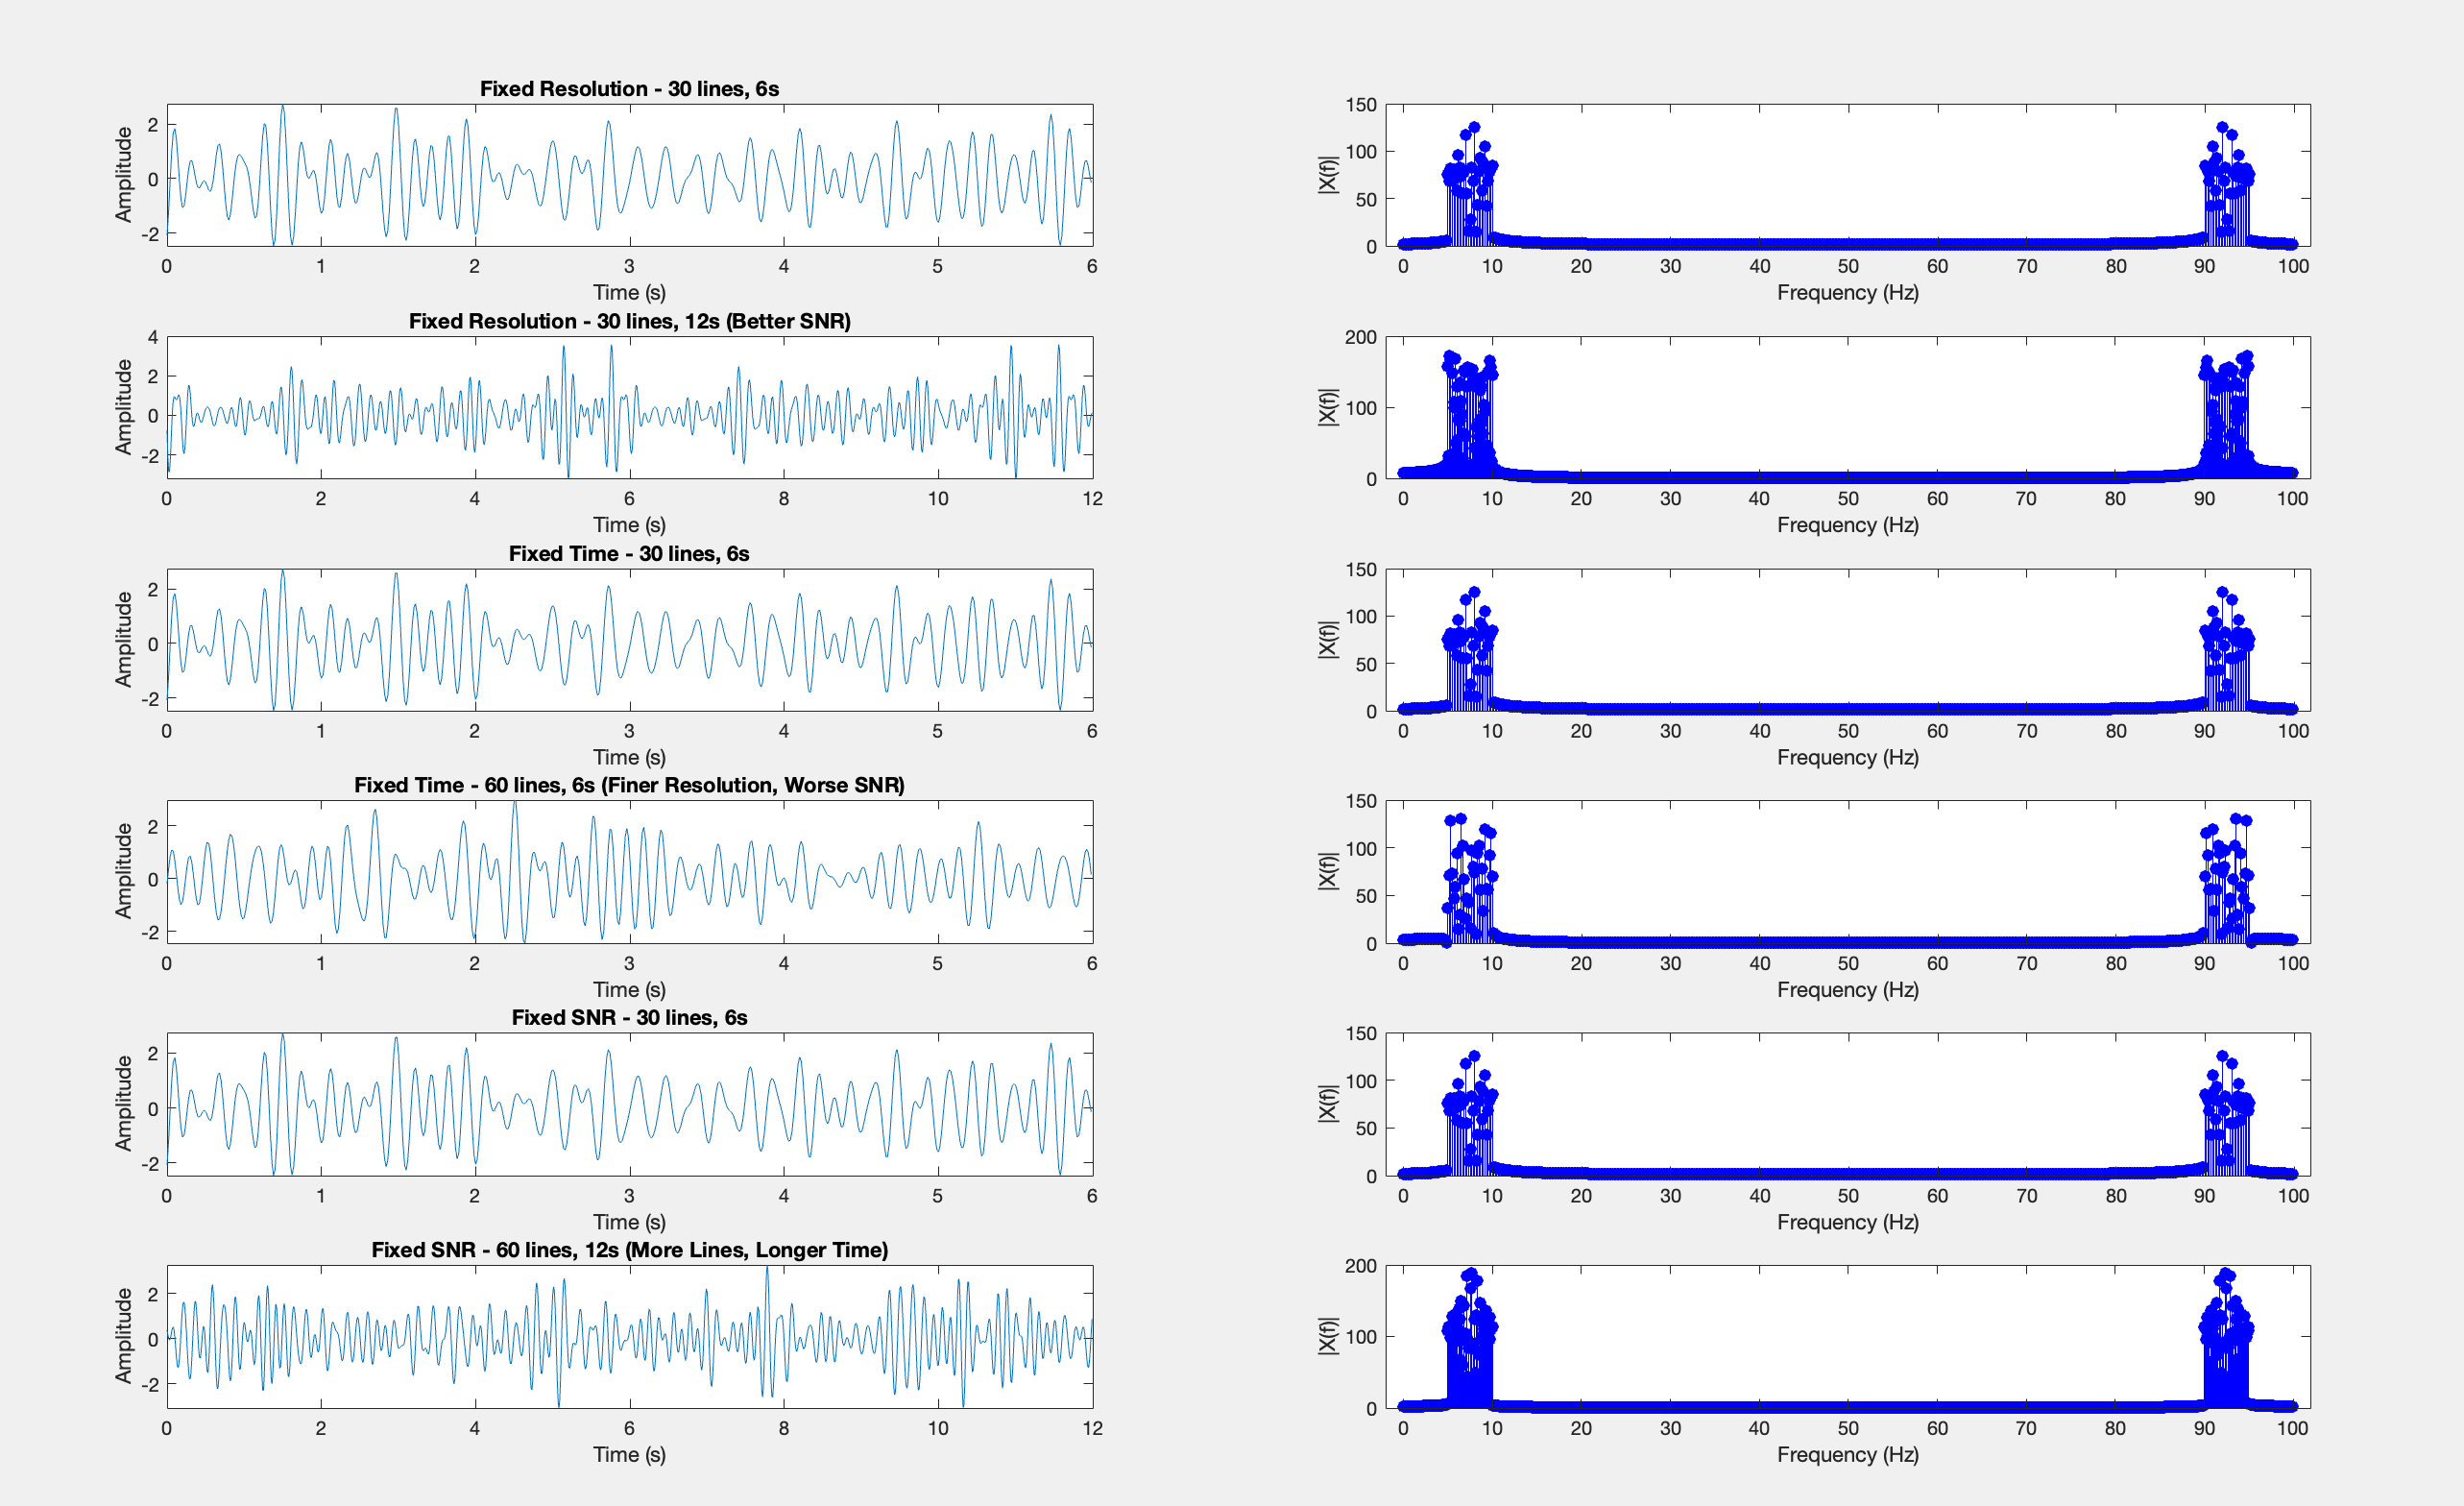
\includegraphics[width=0.9\textwidth]{frf_tradeoff.png}
    \caption{Time and Frequency Domain Plots for Different Multisine Designs Illustrating Trade-offs}
    \label{fig:frf_tradeoff}
\end{figure}

\subsection*{Overview}
Figure \ref{fig:frf_tradeoff} displays the time domain and frequency domain representations of all six multisines. The left column shows the time-domain signals, while the right column shows the corresponding magnitudes of the Discrete Fourier Transform (DFT).

\subsection*{Analysis of Trade-offs}

\subsubsection*{Trade-off 1: Fixed Frequency Resolution}
The first two rows represent cases where 30 equally spaced frequencies between 5 Hz and 10 Hz are excited.
\begin{itemize}
    \item Row 1 uses a 6-second signal.
    \item Row 2 uses a 12-second signal.
\end{itemize}
The longer duration reduces noise variance, improving the SNR. This can be seen from the cleaner peaks in the frequency spectrum of Row 2 compared to Row 1.

\subsubsection*{Trade-off 2: Fixed Measurement Time}
The third and fourth rows correspond to a fixed 6-second measurement duration.
\begin{itemize}
    \item Row 3 excites 30 frequencies.
    \item Row 4 excites 60 frequencies, doubling the resolution.
\end{itemize}
Since the total power (RMS fixed to 1V) must be spread over more frequencies in Row 4, the SNR per frequency decreases. This leads to less distinct peaks in the frequency domain.

\subsubsection*{Trade-off 3: Fixed SNR}
The fifth and sixth rows maintain a constant SNR.
\begin{itemize}
    \item Row 5 excites 30 frequencies over 6 seconds.
    \item Row 6 excites 60 frequencies, requiring the measurement duration to increase to 12 seconds to maintain SNR.
\end{itemize}
This illustrates that improving resolution (more lines) requires a proportional increase in measurement time to maintain SNR.

\subsection*{Summary of Observations}
This experiment confirms the fundamental triangle of FRF trade-offs:
\begin{itemize}
    \item Increasing measurement time allows better SNR at constant resolution.
    \item Increasing frequency resolution reduces SNR if time is fixed.
    \item Maintaining SNR while increasing resolution requires longer measurement time.
\end{itemize}
The ability to choose optimal parameters depends on the specific constraints of the experiment (available time, acceptable noise, required resolution).

\section*{MATLAB Code Implementation}
The MATLAB code used to generate these results is included below:

\lstset{language=Matlab, basicstyle=\ttfamily\small, breaklines=true}
\begin{lstlisting}
% Tradeoff in FRF Measurement - MATLAB Assignment
clc; clear; close all;

fs = 100;            % Sampling frequency (Hz)
RMS_des = 1;         % Desired RMS value
f_start = 5;         % Start frequency (Hz)
f_end = 10;          % End frequency (Hz)

% Trade-off 1: Fixed Frequency Resolution
N1 = fs * 6; % 6s
frequencies1 = linspace(f_start, f_end, 30);
x1 = generate_multisine(N1, frequencies1, fs, RMS_des);

N2 = fs * 12; % 12s
x2 = generate_multisine(N2, frequencies1, fs, RMS_des);

% Trade-off 2: Fixed Measurement Time
x3 = x1; % Same as Fixed Resolution 1
frequencies4 = linspace(f_start, f_end, 60);
x4 = generate_multisine(N1, frequencies4, fs, RMS_des);

% Trade-off 3: Fixed SNR
x5 = x1;
x6 = generate_multisine(N2, frequencies4, fs, RMS_des);

% Function to generate multisine
function x = generate_multisine(N, frequencies, fs, RMS_des)
    t = (0:N-1) / fs;
    x = zeros(1, N);
    for f = frequencies
        phase = 2*pi*rand();
        x = x + cos(2*pi*f*t + phase);
    end
    x = x * (RMS_des / rms(x));
end
\end{lstlisting}

\section*{Conclusion}
This assignment provides a hands-on demonstration of how measurement time, frequency resolution, and SNR are interrelated in FRF measurements. The design of an optimal multisine excitation depends on the specific measurement goals whether the priority is fast measurement, high resolution, or high SNR. Understanding these trade-offs is essential for practical system identification and experimental design.

\end{document}